\documentclass[border=2pt]{standalone}
\usepackage[T1]{fontenc}
\usepackage{mathptmx}
\usepackage{tikz}
\usetikzlibrary{arrows.meta,positioning,fit,calc,shapes.geometric,backgrounds}
\usepackage{siunitx}
\tikzset{
  >={Stealth[length=1.8mm]},
  blk/.style={draw, thick, minimum height=11mm, text width=16mm, align=center, font=\scriptsize, inner sep=1.5pt, fill=white},
  lab/.style={font=\scriptsize, align=center},
  every picture/.style={line width=0.6pt},
}

% One-column version (about 75 mm wide): signal path top to bottom on the left,
% UART controller on the right with its three test paths (D, T, C).
\begin{document}
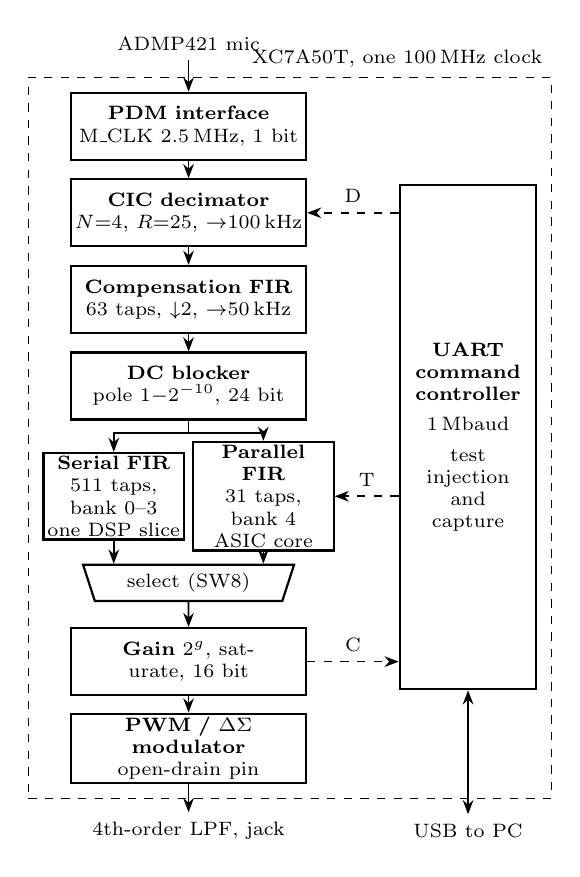
\begin{tikzpicture}[
  vb/.style={draw, thick, minimum height=8.5mm, text width=29mm, align=center, font=\scriptsize, inner sep=1.2pt, fill=white},
  fb/.style={draw, thick, minimum height=10mm, text width=17mm, align=center, font=\scriptsize, inner sep=1.2pt, fill=white}]
\node[lab] (mic) at (0,0) {ADMP421 mic};
\node[vb] (pdm)  at (0,-1.05) {\textbf{PDM interface}\\M\_CLK \SI{2.5}{MHz}, 1 bit};
\node[vb] (cic)  at (0,-2.15) {\textbf{CIC decimator}\\$N{=}4$, $R{=}25$, $\to$\SI{100}{kHz}};
\node[vb] (comp) at (0,-3.25) {\textbf{Compensation FIR}\\63 taps, $\downarrow$2, $\to$\SI{50}{kHz}};
\node[vb] (dc)   at (0,-4.35) {\textbf{DC blocker}\\pole $1{-}2^{-10}$, 24 bit};
\node[fb] (fir)  at (-0.95,-5.75) {\textbf{Serial FIR}\\511 taps, bank 0--3\\one DSP slice};
\node[fb] (par)  at ( 0.95,-5.75) {\textbf{Parallel FIR}\\31 taps, bank 4\\ASIC core};
\node[draw, thick, trapezium, trapezium angle=72, minimum width=27mm, minimum height=4.5mm, inner sep=1pt,
      font=\scriptsize, fill=white, shape border rotate=180] (mux) at (0,-6.85) {select (SW8)};
\node[vb] (gain) at (0,-7.85) {\textbf{Gain} $2^g$, saturate, 16 bit};
\node[vb] (dac)  at (0,-8.95) {\textbf{PWM / $\Delta\Sigma$ modulator}\\open-drain pin};
\node[lab] (lpf) at (0,-10.0) {4th-order LPF, jack};
\draw[->] (mic) -- (pdm); \draw[->] (pdm) -- (cic); \draw[->] (cic) -- (comp); \draw[->] (comp) -- (dc);
\coordinate (sp) at (0,-4.95);
\draw (dc.south) -- (sp);
\draw[->] (sp) -| (fir.north);
\draw[->] (sp) -| (par.north);
\draw[->] (fir.south) -- (fir.south |- mux.north);
\draw[->] (par.south) -- (par.south |- mux.north);
\draw[->] (mux) -- (gain); \draw[->] (gain) -- (dac); \draw[->] (dac) -- (lpf);
% ---- UART controller
\node[draw, thick, text width=15mm, align=center, font=\scriptsize, fill=white, minimum height=64mm] (cmd) at (3.55,-5.0)
      {\textbf{UART\\command\\controller}\\[3pt]\SI{1}{Mbaud}\\[3pt]test\\injection\\and\\capture};
\node[lab] (host) at (3.55,-10.0) {USB to PC};
\draw[<->] (cmd.south) -- (host.north);
\draw[->, dashed] (cic.east -| cmd.west) -- node[lab, above]{D} (cic.east);
\draw[->, dashed] (par.east -| cmd.west) -- node[lab, above]{T} (par.east);
\draw[->, dashed] (gain.east) -- node[lab, above]{C} (gain.east -| cmd.west);
\begin{scope}[on background layer]
\node[draw, dashed, fit=(pdm)(fir)(par)(dac)(cmd), inner sep=1.8mm] (fpga) {};
\end{scope}
\node[lab, anchor=south east] at (fpga.north east) {XC7A50T, one \SI{100}{MHz} clock};
\end{tikzpicture}
\end{document}
